\section{Dashboard Design Rationale and Usability}\label{sec:dash}
The dashboard (D3.js v7, no other charting library) is built for decision-makers who are not data scientists. Each view answers one question and all views share one state object, so selecting a district, a disease or a time range in any view filters or highlights all others (Fig.~\ref{fig:dash}).
\begin{figure*}[t]\centering
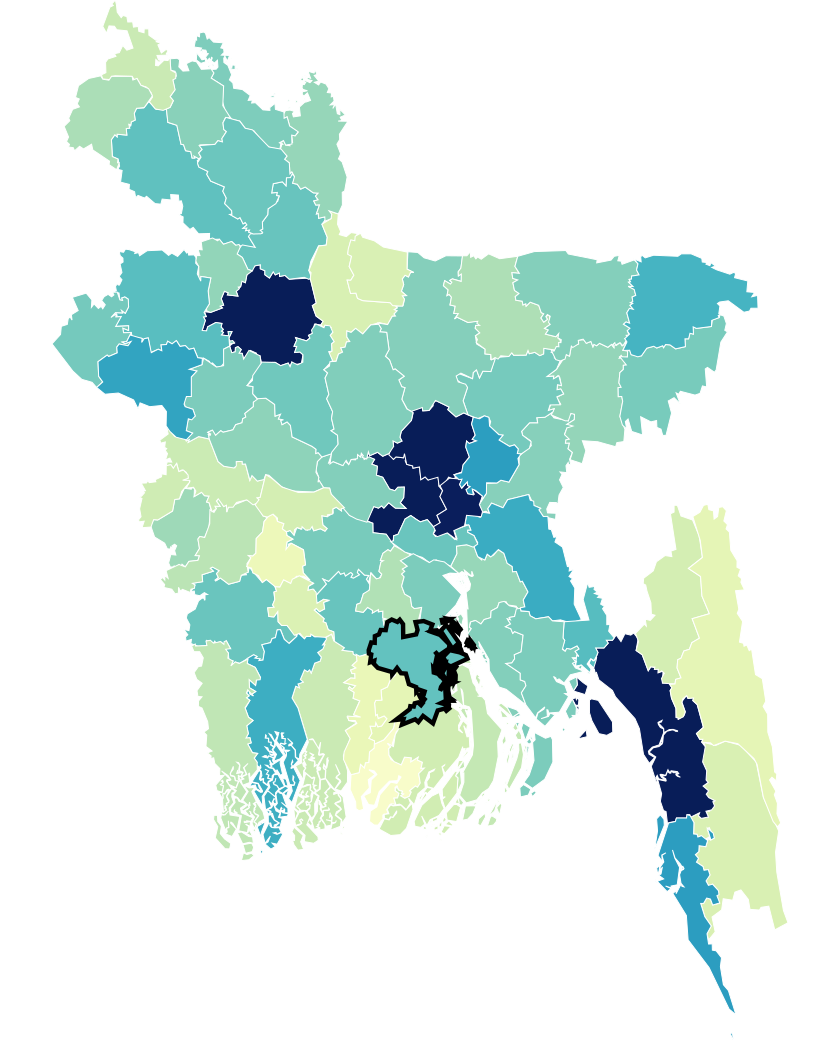
\includegraphics[width=0.30\textwidth]{figures/dash_map.png}\hfill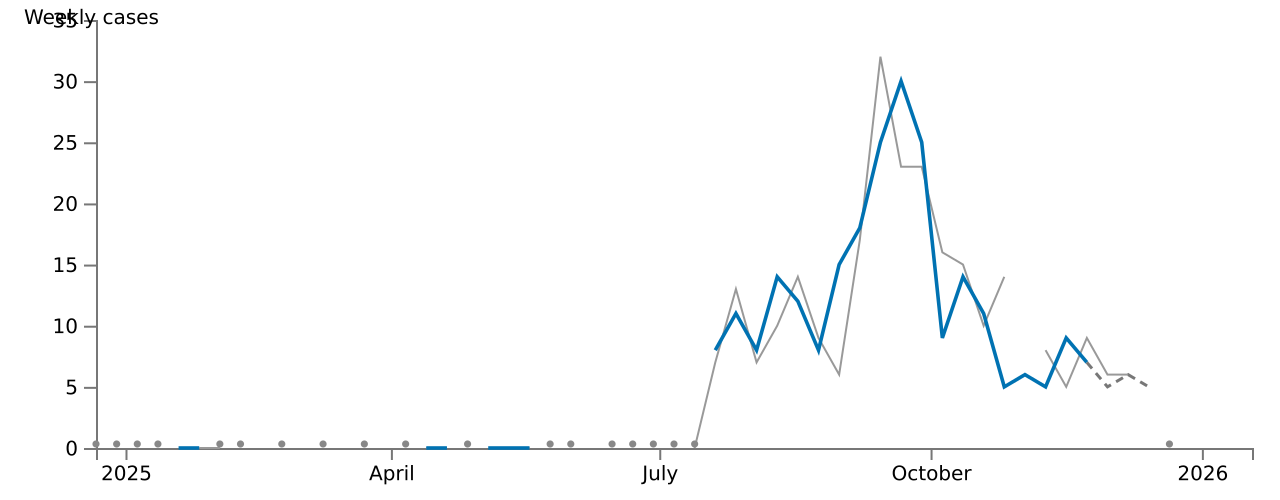
\includegraphics[width=0.66\textwidth]{figures/dash_ts.png}\\[2pt]
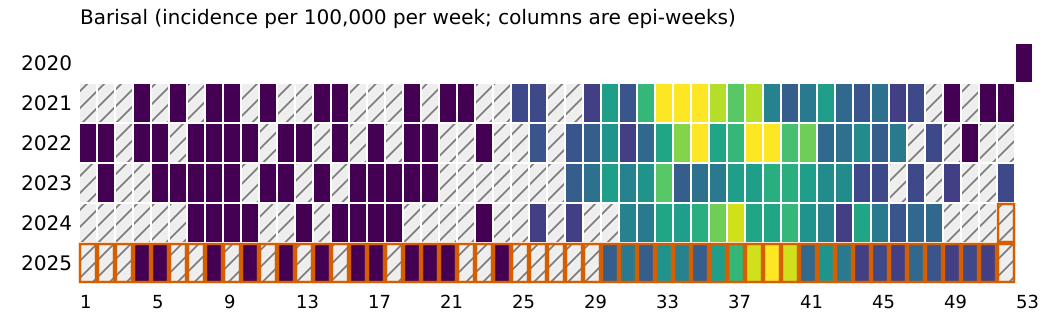
\includegraphics[width=0.48\textwidth]{figures/dash_heat.png}\hfill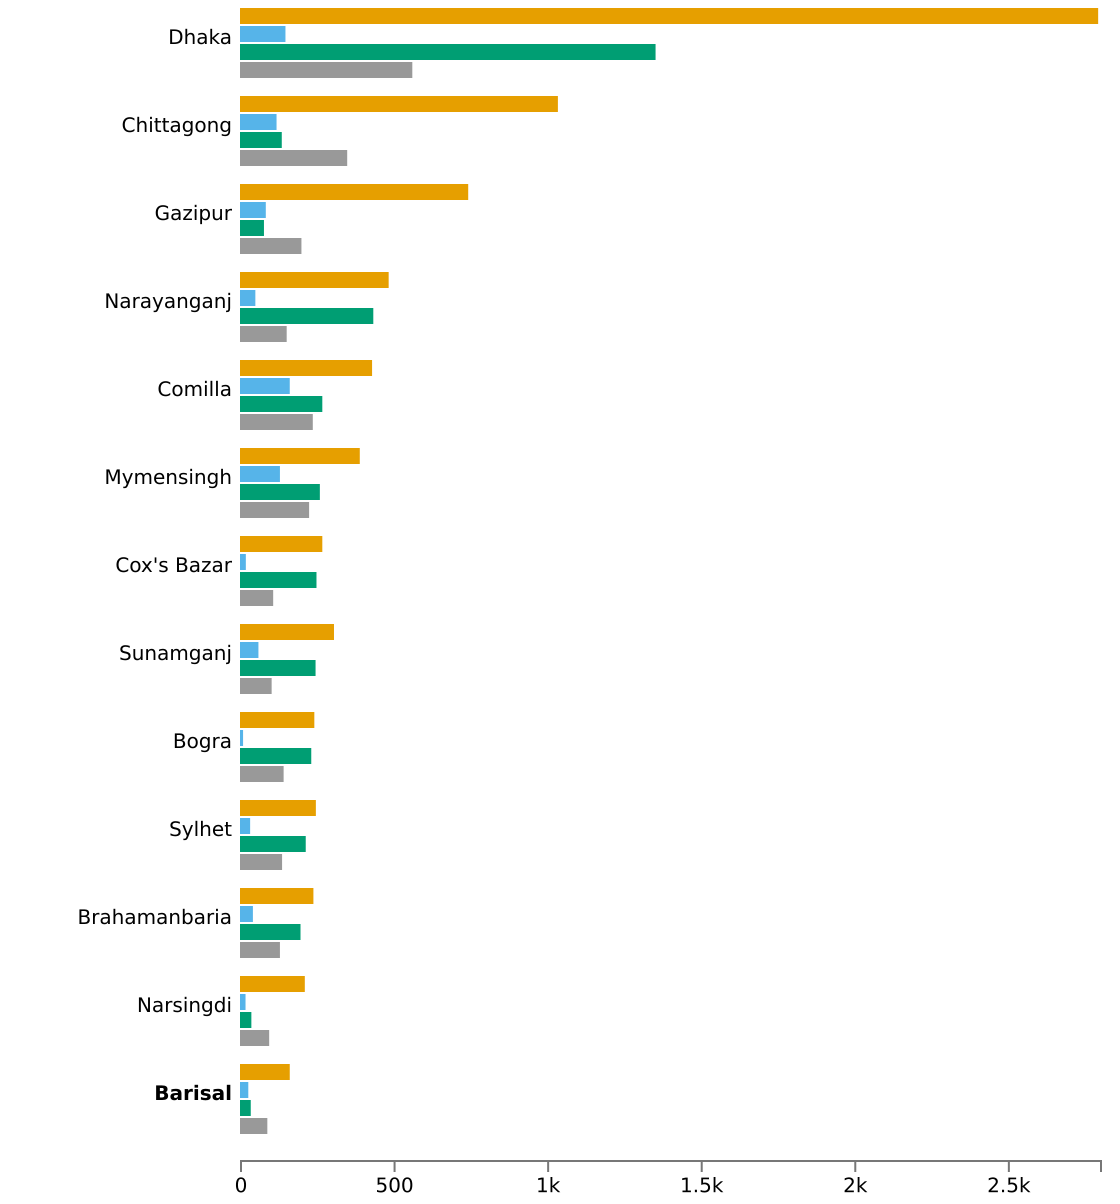
\includegraphics[width=0.48\textwidth]{figures/dash_alloc.png}
\caption{Views 1 to 4 rendered from the dashboard code on the exported data (jsdom rendering, no browser available in the build environment). Top: incidence map with the selected district outlined, and the time series for that district (blue: cases by onset week; grey: cases as reported; dashed tail: weeks with late reports pending; grey dots: suppressed weeks). Bottom: seasonal heatmap by year and epi-week, and demand, stock and recommended allocation.}\label{fig:dash}\end{figure*}

\textbf{The five required views.} (1) A district choropleth of incidence per 100\,000 for the brushed time range, with triangular markers for districts in alert and hatching for suppressed values. (2) A time series for the selected district (or the whole country) with cases by onset week, cases as reported (the basis of alerts), the 80\% forecast band for the next four weeks, the alert threshold line and alert markers; a brush on the context chart sets the time range for every view. (3) A seasonal heatmap, either year by epi-week for the selected district or all districts by epi-week. (4) An allocation view comparing forecast upper demand, current stock, recommended allocation and the population-proportional baseline for a chosen resource. (5) A ranked early-warning table of districts by alert score, with reported cases, alert status, four-week forecast and bed gap. Beyond the required views the page has a data-quality panel, the seasonal preparedness calendar, and a what-if panel.

\textbf{What-if panel (VIS-5).} Sliders set the budget, the equity floor and the detection threshold. Allocations come from a precomputed grid of 25 scenarios (five budgets times five values of $\alpha$), and alerts are recomputed in the browser from the stored scores, so no server is needed. Two small charts show where the current setting sits on the efficiency--equity curve and on the detection trade-off curve, which lets a user see what a change costs before making it.

\textbf{Scale-aware design (VIS-4).} The browser loads only aggregated, suppressed JSON: @@DASH_SIZE@@; never line-level data. The national bundle holds district by disease by week counts (64 districts by 4 diseases by about 260 weeks), detection scores for the last 104 weeks, the four-week forecasts and the allocation grid. A district officer's browser loads a division-level file (aggregates only) and the file of their own district. Aggregation to districts and weeks was chosen because it is the finest level at which most cells exceed the suppression limit (Section~\ref{sec:cep}) and the level at which decisions are made.

\textbf{Honest design (VIS-6).} Palettes are colour-blind safe (ColorBrewer YlGnBu, viridis and the Okabe--Ito set), every symbol is also coded by shape or pattern (triangles for alerts, hatching for suppressed cells), forecasts are never shown without their band, weeks whose counts are still incomplete are drawn dashed and labelled, and every panel carries the data-freshness stamp (latest report date, build time, forecast origin).

\textbf{Verification.} A headless test loads the dashboard in jsdom against the exported data, checks that all views draw (64 districts, ranking rows, heatmap cells, allocation bars, what-if charts, calendar), exercises linked selection, all diseases, all three alert methods, both heatmap layouts, brushing, the what-if sliders and the district-officer role, and fails on any script error. It passes. It cannot judge legibility or layout in a real browser.

\textbf{Usability study.} The assignment requires a check with at least two non-computer-science users. @@USABILITY@@
